\section{Architecture Overview}

\begin{frame}\frametitle{Architecture Overview}

\begin{enumerate} 

  \footnotesize
  
  \li{morpheus-graphql-core} low level functionalities and common types, such as  parsing, pretty-printing, validation, ast AST for the GraphQL schema and query language.

  \li{morpheus-graphql-client} Enables type-safe client queries. It generates the query and response types on valid queries but throws a compilation error on the invalid query.

  \li{morpheus-graphql-app} utilities for creating executable GraphQL applications. primary task is to execute the GraphQL document representations. 
  
  \li{morpheus-graphql-subscriptions} Takes argument \expr{App} and generates  WebSockets server based on it. It is independent of the server package and accepts any \expr{App} derived from an arbitrary server.

  \li{morpheus-graphql} derives executable \expr{App} with native Haskell types by mapping them to GraphQL representations. derived application can be executed by app and subscriptions packages.

  % This package also leverages Template Haskell and enables importing type definitions from the GraphQL schema. In particular, the \expr{importGQLDocument} function defines corresponding native Haskell types for each GraphQL type. Users can then provide resolver values for these types, from which the Morpheus compiler derives a server application. 
  % This package also provides the function \expr{compileTimeSchemaValidation} for compile-time schema validation, which checks if the API definition represents a valid GraphQL schema.

\end{enumerate}

\end{frame}

\begin{frame}
%!TEX root = ../../main.tex

\begin{figure}
\caption{
    Dependency Graph of the Morpheus GraphQL Packages
    \label{fig:dependency-graph}
    }
\begin{center}
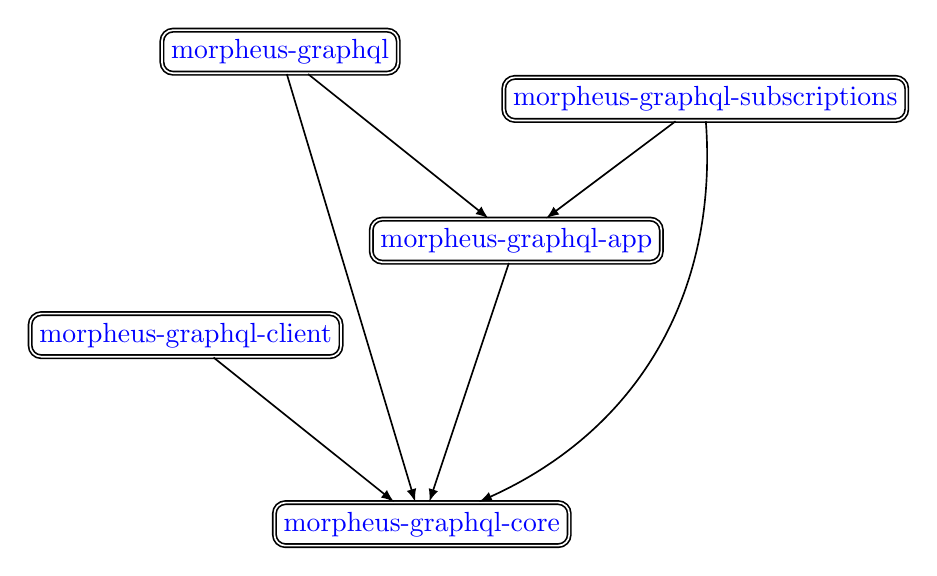
\begin{tikzpicture}[
        scale=.6,
        auto=left,
        -latex ,
        auto ,
        node distance =2 cm and 2cm ,
        % on grid ,
        semithick ,
        package/.style ={ fill=red!20,draw,double,rounded corners ,top color =white ,draw , text=blue , minimum width =1 cm},
    ] 
    \node[package] (core) at (10,0) {morpheus-graphql-core};
    \node[package] (client) at (5,4)  {morpheus-graphql-client};
    \node[package] (app) at (12,6)  {morpheus-graphql-app};
    \node[package] (server) at (7,10)  {morpheus-graphql};
    \node[package] (subs) at (16,9) {morpheus-graphql-subscriptions};
  
    \path (client) edge (core);
    \path (app)  edge (core);
    \path (server)  edge  (core);
    \path (server)  edge  (app);
    \path (subs)  edge  (app);
    \path 
        (subs) 
            edge [bend left =35] 
        (core);  

\end{tikzpicture}
\end{center}
\end{figure}

\end{frame}
